\documentclass[tikz,border=0pt]{standalone}
\pdfminorversion=7
\usepackage[T1]{fontenc}
\usepackage{lmodern,amsmath,amssymb,graphicx}
\usepackage{pgfplots}
\usetikzlibrary{arrows.meta,calc,positioning,patterns,decorations.pathreplacing}
\pgfplotsset{compat=1.18}
\definecolor{family}{RGB}{0,140,18}
\definecolor{familypale}{RGB}{225,255,226}
\definecolor{frozen}{RGB}{49,57,208}
\definecolor{frozenpale}{RGB}{234,235,255}
\definecolor{adapter}{RGB}{219,102,0}
\definecolor{adapterpale}{RGB}{255,196,135}
\definecolor{outputcol}{RGB}{120,38,130}
\definecolor{ink}{RGB}{33,33,33}
\definecolor{muted}{RGB}{105,105,105}
\tikzset{
 figure/.style={x=1pt,y=1pt,line cap=round,line join=round,text=ink,
   >={Stealth[length=7pt,width=6pt]},font=\fontsize{20}{24}\selectfont},
 title/.style={font=\fontsize{29}{33}\selectfont},
 heading/.style={font=\fontsize{22}{26}\selectfont},
 labeltext/.style={font=\fontsize{18}{22}\selectfont,align=center},
 smalllabel/.style={font=\fontsize{15}{19}\selectfont,align=center},
 equation/.style={font=\fontsize{24}{29}\selectfont,align=center},
 flow/.style={->,line width=1.3pt},
 fineflow/.style={->,line width=.8pt},
 target/.style={circle,fill=family,draw=white,line width=1.2pt,inner sep=0pt,minimum size=12pt},
 candidate/.style={circle,fill=white,draw=muted,line width=1.3pt,inner sep=0pt,minimum size=10pt},
 neuron/.style={circle,draw=frozen,fill=frozen!18,minimum size=13pt,inner sep=0pt,line width=.8pt}
}
\DeclareMathOperator{\rank}{rank}
\DeclareMathOperator{\row}{row}
\DeclareMathOperator{\col}{col}
\newcommand{\R}{\mathbb R}
\graphicspath{{assets/}}
\newcommand{\canvas}[1]{\path[use as bounding box] (0,0) rectangle (960,600);
  \node[title,anchor=west] at (36,557) {#1};}
\newcommand{\glyphgrid}[2]{
 \begin{scope}[shift={(#1,#2)}]
  \fill[white] (0,0) rectangle (136,136);
  \foreach \x/\y/\c in {1/1/80,2/2/80,2/3/45,3/4/45,3/5/45,4/5/100,4/6/45,5/6/45,5/4/45,5/2/100,6/1/80}{
    \fill[frozen!\c] (\x*17,\y*17) rectangle ++(17,17);
  }
  \draw[step=17pt,black!30,line width=.35pt] (0,0) grid (136,136);
  \draw[black!45,line width=.6pt] (0,0) rectangle (136,136);
 \end{scope}}

\begin{document}
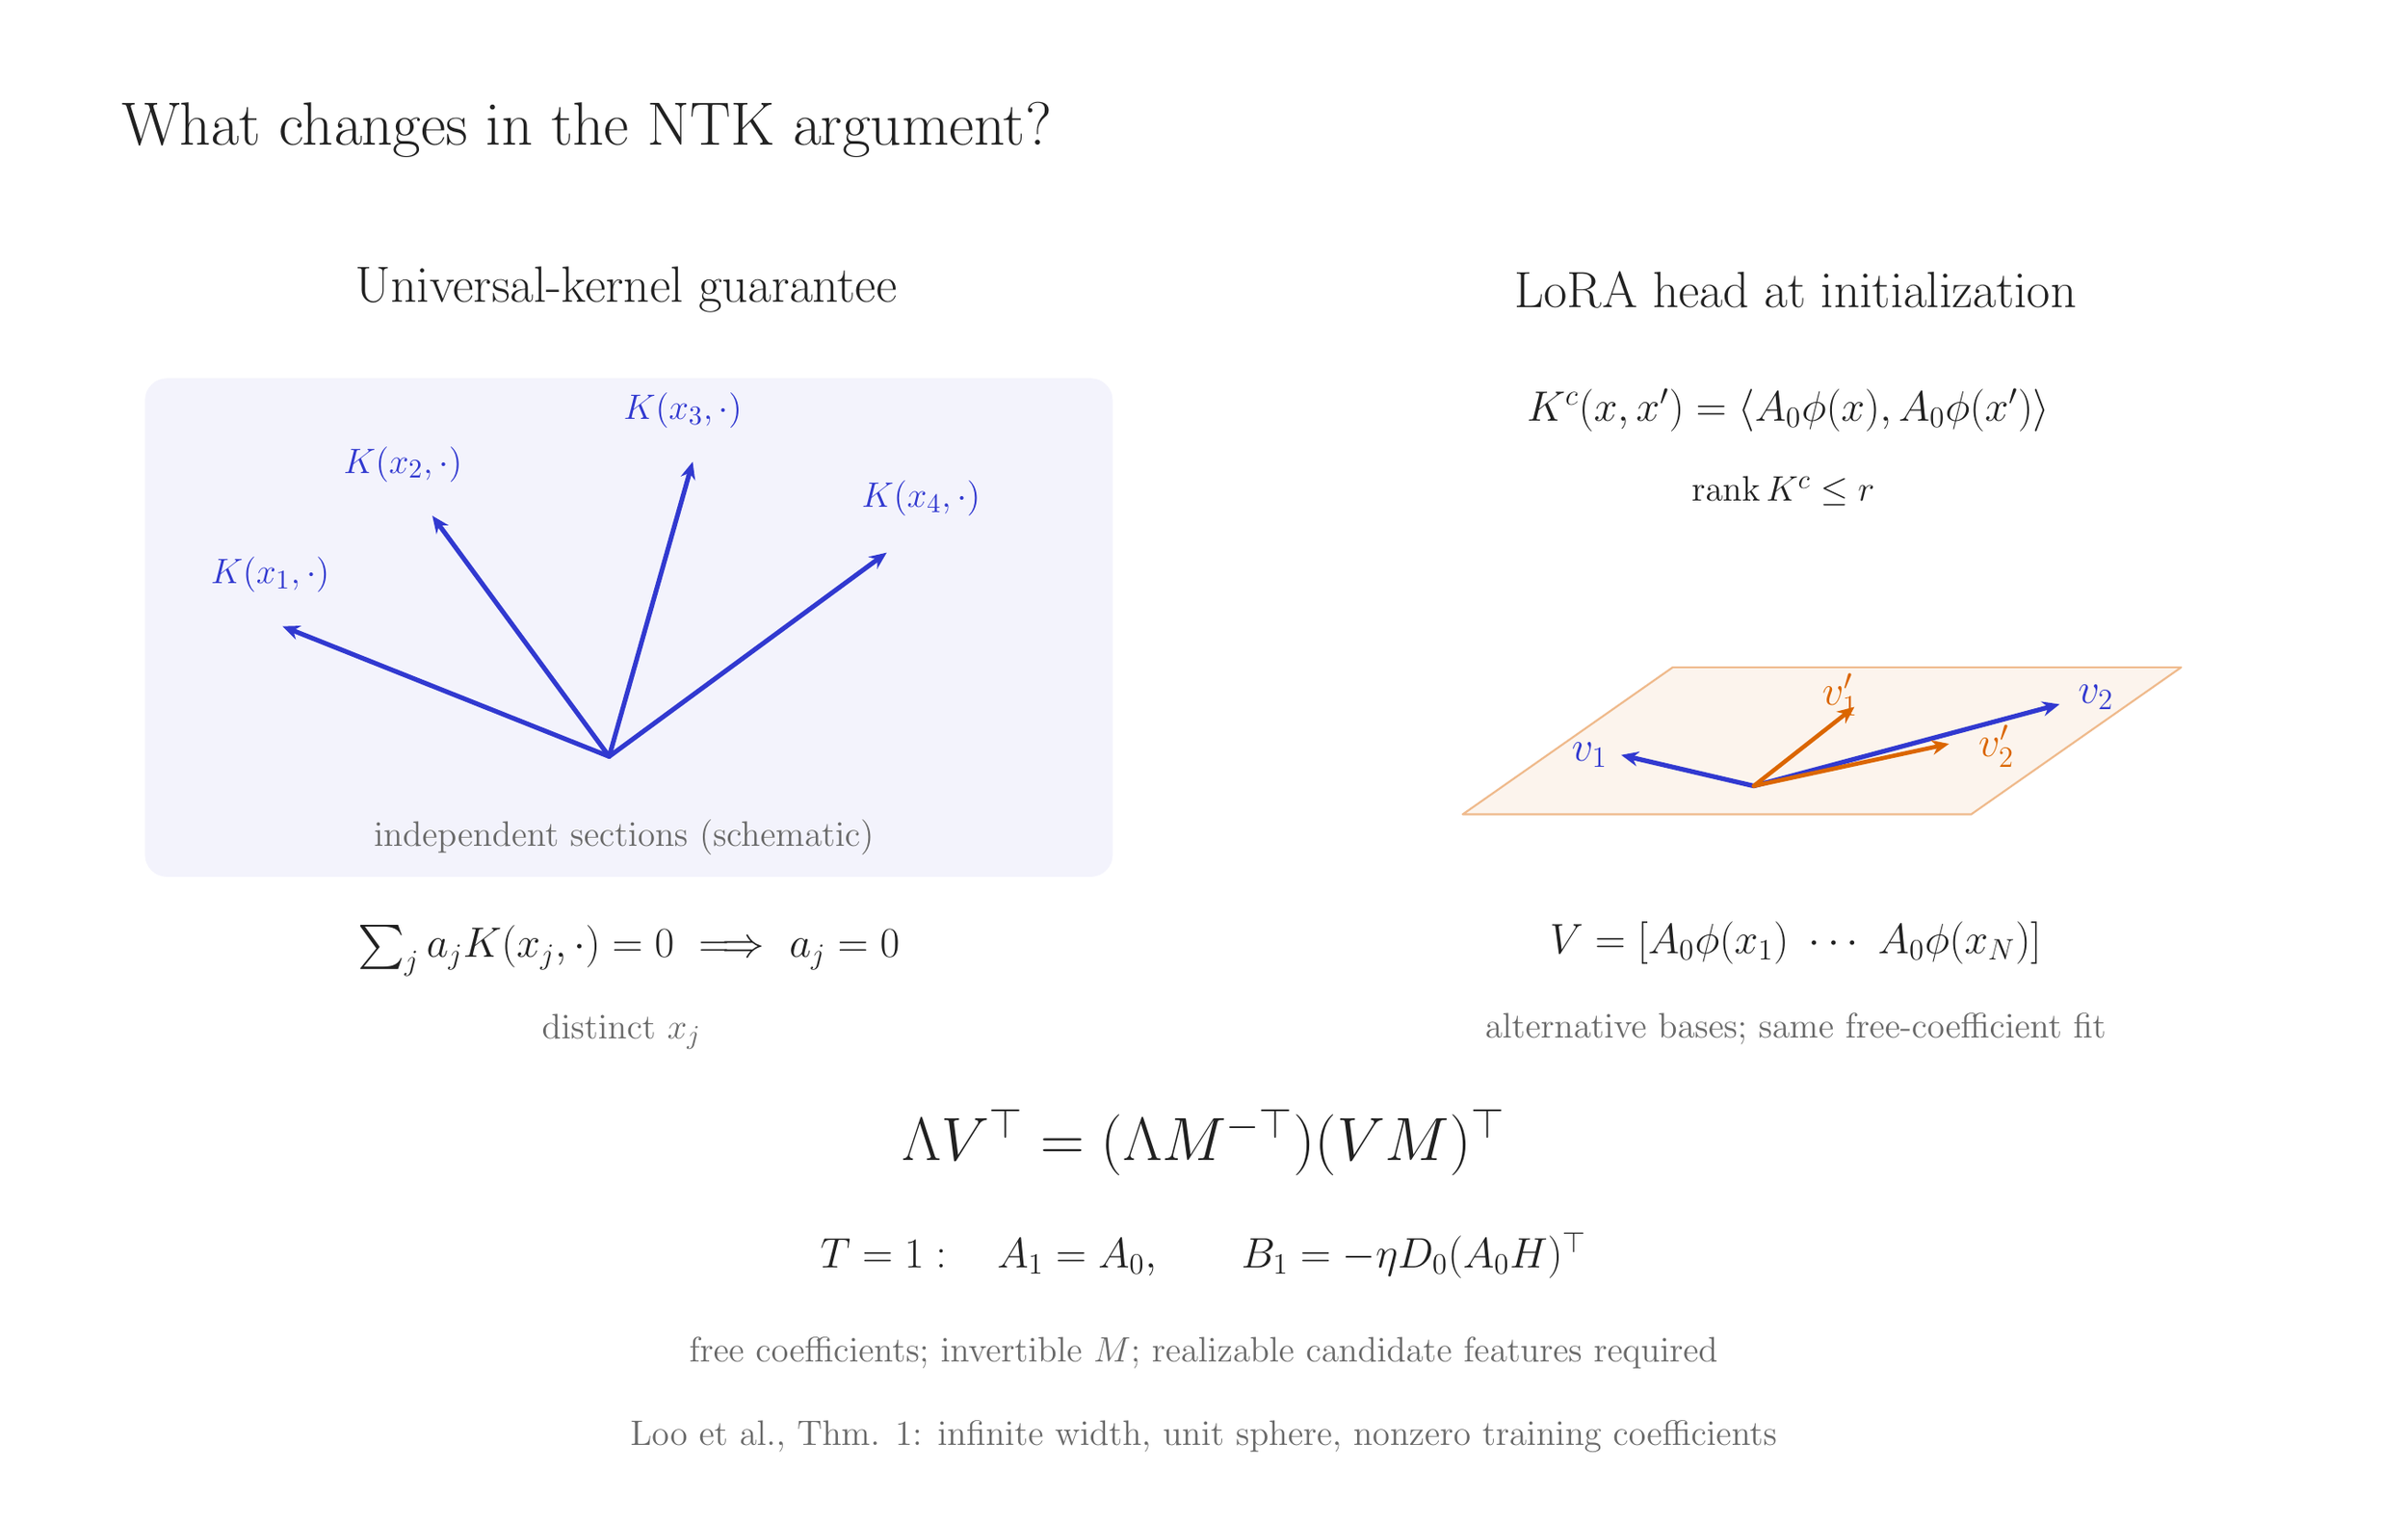
\begin{tikzpicture}[figure]
\canvas{What changes in the NTK argument?}
\node[heading] at (245,492) {Universal-kernel guarantee};
\node[heading] at (721,492) {LoRA head at initialization};
\fill[frozen!6,rounded corners=9pt] (49,253) rectangle (443,456);
\begin{scope}[shift={(238,302)}]
 \draw[flow,frozen,line width=1.9pt] (0,0)--(-133,53);
 \draw[flow,frozen,line width=1.9pt] (0,0)--(-72,98);
 \draw[flow,frozen,line width=1.9pt] (0,0)--(34,120);
 \draw[flow,frozen,line width=1.9pt] (0,0)--(113,83);
 \node[smalllabel,text=frozen] at (-138,74) {$K(x_1,\cdot)$};
 \node[smalllabel,text=frozen] at (-84,119) {$K(x_2,\cdot)$};
 \node[smalllabel,text=frozen] at (30,141) {$K(x_3,\cdot)$};
 \node[smalllabel,text=frozen] at (127,105) {$K(x_4,\cdot)$};
\end{scope}
\node[smalllabel,text=muted] at (244,269) {independent sections (schematic)};
\node[labeltext] at (246,223) {$\sum_j a_jK(x_j,\cdot)=0\ \Longrightarrow\ a_j=0$};
\node[smalllabel,text=muted] at (243,190) {distinct $x_j$};
\node[labeltext] at (718,443) {$K^c(x,x')=\langle A_0\phi(x),A_0\phi(x')\rangle$};
\node[smalllabel] at (716,410) {$\rank K^c\le r$};
\begin{scope}[shift={(704,290)},x={(1pt,0pt)},y={(.5pt,.35pt)}]
 \filldraw[fill=adapter!7,draw=adapter!45,line width=.8pt]
  (-102,-33)--(105,-33)--(105,138)--(-102,138)--cycle;
 \draw[flow,frozen,line width=1.9pt] (0,0)--(-72,36);
 \draw[flow,frozen,line width=1.9pt] (0,0)--(77,95);
 \draw[flow,adapter,line width=1.7pt] (0,0)--(-5,92);
 \draw[flow,adapter,line width=1.7pt] (0,0)--(55,49);
 \node[labeltext,text=frozen,anchor=east] at (-74,36) {$v_1$};
 \node[labeltext,text=frozen,anchor=west] at (77,103) {$v_2$};
 \node[labeltext,text=adapter,anchor=east] at (-7,106) {$v'_1$};
 \node[labeltext,text=adapter,anchor=west] at (65,46) {$v'_2$};
\end{scope}
\node[labeltext] at (721,226) {$V=[A_0\phi(x_1)\ \cdots\ A_0\phi(x_N)]$};
\node[smalllabel,text=muted] at (721,191) {alternative bases; same free-coefficient fit};
\node[equation] at (480,145) {$\Lambda V^\top=(\Lambda M^{-\top})(VM)^\top$};
\node[labeltext] at (480,99) {$T=1:\quad A_1=A_0,\qquad B_1=-\eta D_0(A_0H)^\top$};
\node[smalllabel,text=muted] at (480,59) {free coefficients; invertible $M$; realizable candidate features required};
\node[smalllabel,text=muted] at (480,25) {Loo et al., Thm. 1: infinite width, unit sphere, nonzero training coefficients};
\end{tikzpicture}
\end{document}
